\section{Příklad 1}
% Jako parametr zadejte skupinu (A-H)
\prvniZadani{D}

\section*{Riešenie}
\subsection*{1. krok}
Spojíme paralélne zapojené rezistory $R_5$ a $R_6$.
Taktiež spojíme sériovo zapojené rezistory $R_7$ a $R_8$.\\
\begin{center}
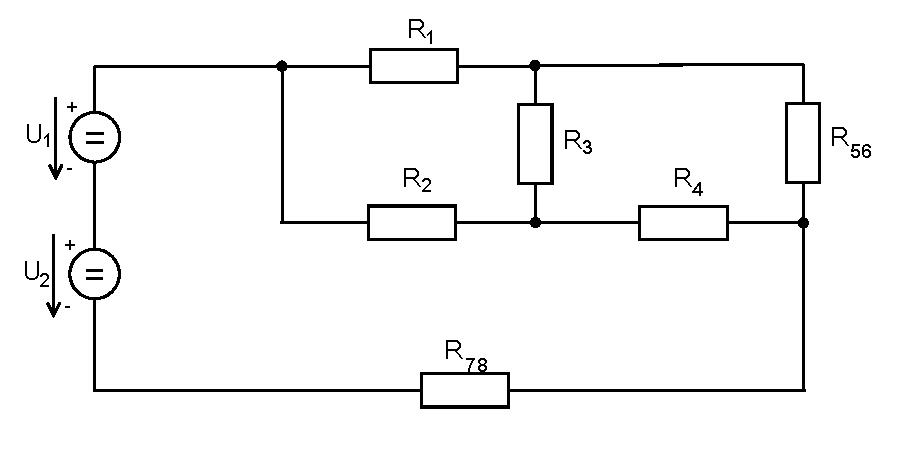
\includegraphics[scale=0.9,keepaspectratio]{xbednar00/zdroje/pr1/pr1_krok1.pdf}
\end{center}

$$R_{56}=\frac{R_5*R_6}{R_5+R_6}\doteq215,7843\Omega$$\\
$$R_{78}=R_7+R_8=440\Omega$$

\newpage
\subsection*{2. krok}
Použijeme transfiguráciu z trojuholníka na hviezdu medzi rezistormi $R_1$, $R_2$ a $R_3$.
\begin{center}
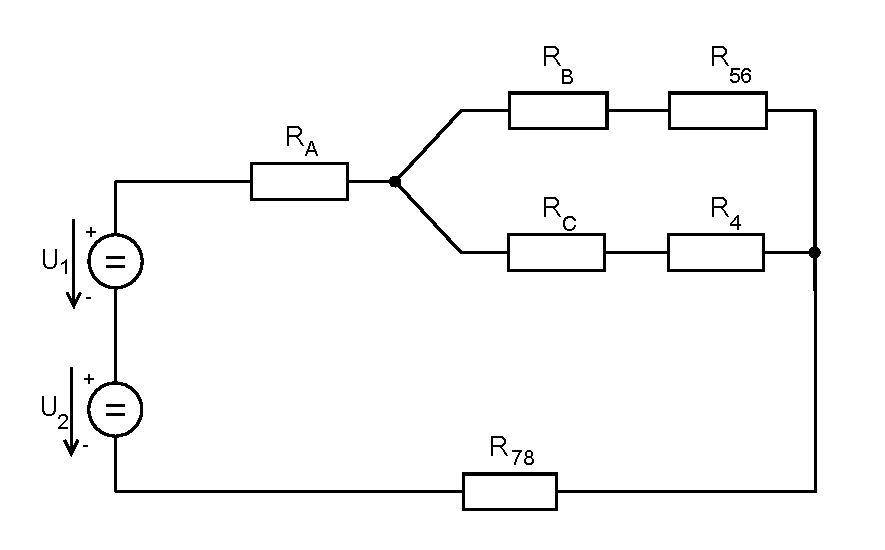
\includegraphics[scale=0.75,keepaspectratio]{xbednar00/zdroje/pr1/pr1_krok2.pdf}
\end{center}
$$R_A=\frac{R_1*R_2}{R_1+R_2+R_3}\doteq237,9191\Omega$$\\
$$R_B=\frac{R_1*R_3}{R_1+R_2+R_3}\doteq80,1156\Omega$$\\
$$R_C=\frac{R_2*R_3}{R_1+R_2+R_3}\doteq186,9364\Omega$$\\

\subsection*{3. krok}
Spojíme dvojice sériovo zapojených  rezistorov $R_B$ s $R_{56}$ a $R_C$ s $R_4$.
\begin{center}
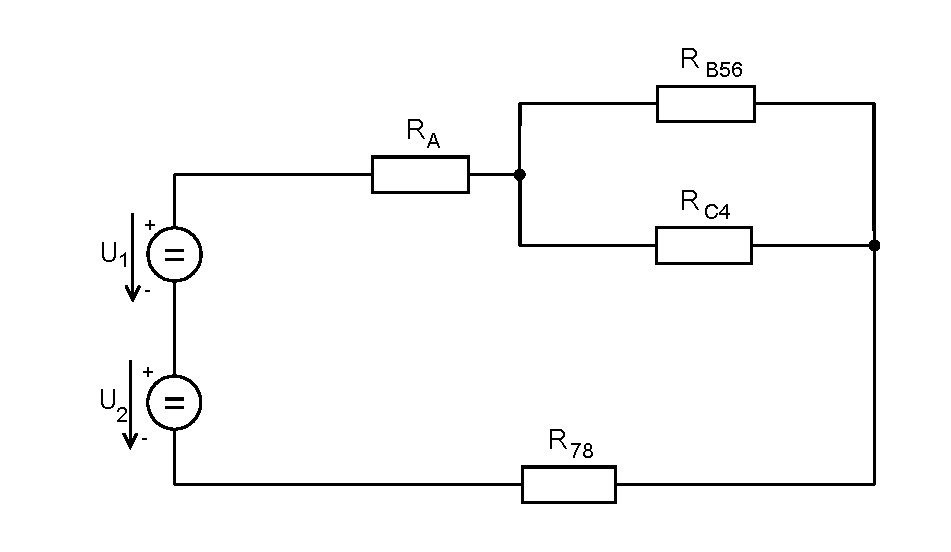
\includegraphics[scale=0.75,keepaspectratio]{xbednar00/zdroje/pr1/pr1_krok3.pdf}
\end{center}
$$R_{B56}=R_B+R_{56}\doteq295,8999\Omega$$
$$R_{C4}=R_C+R_4\doteq466,9364\Omega$$

\subsection*{4. krok}
Spojíme paralélne zapojené  rezistory $R_{B56}$ a $R_{C4}$.
\begin{center}
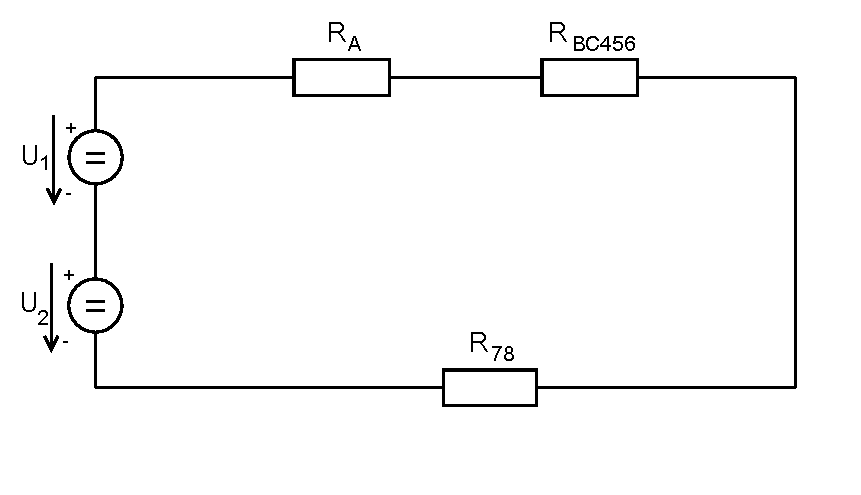
\includegraphics[scale=0.8,keepaspectratio]{xbednar00/zdroje/pr1/pr1_krok4.pdf}
\end{center}
$$R_{BC456}=\frac{R_{B56}*R_{C4}}{R_{B56}+R_{C4}}\doteq181,1220\Omega$$\\

\subsection*{5. krok}
Spojením 3 rezistorov $R_A$, $R_{BC456}$ a $R_{78}$ dostaneme výsledný odpor $R_{EKV}$.
Následne dopočítame $I$.
\begin{center}
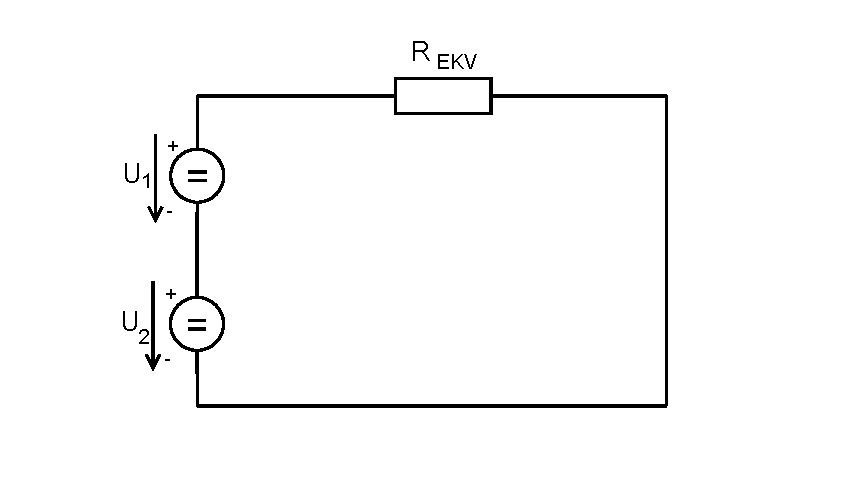
\includegraphics[scale=0.8,keepaspectratio]{xbednar00/zdroje/pr1/pr1_krok5.pdf}
\end{center}
$$R_{EKV}=R_A+R_{BC456}+R_{78}\doteq859,0411\Omega$$\\ 
$$I=\frac{U_1+U_2}{R_{EKV}}\doteq0,2212A$$

\newpage
\subsection*{6. krok}
Teraz budeme obvod rozkladať opačným smerom. Kedže poznáme prúd $I$, tak môžeme vypočítať napätie na rezistoroch $R_A$ a $R_{BC456}$.
\begin{center}
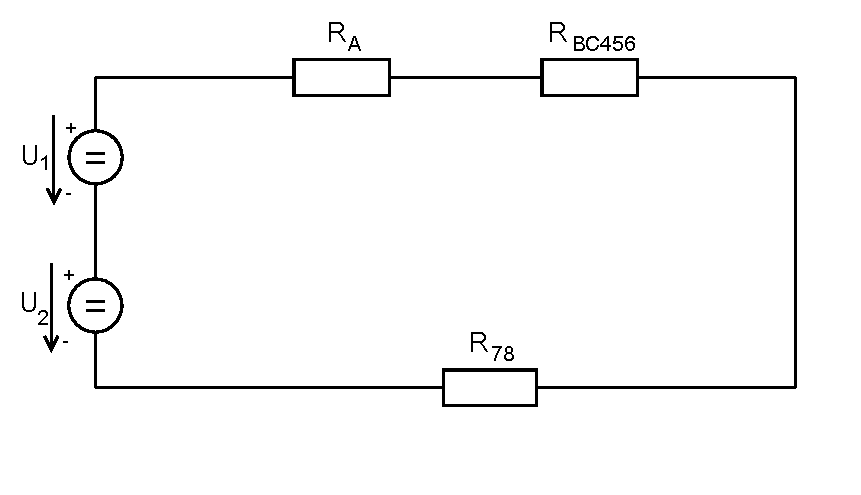
\includegraphics[scale=0.75,keepaspectratio]{xbednar00/zdroje/pr1/pr1_krok6.pdf}
\end{center}
$$U_{R_{BC456}}=I*R_{BC456}\doteq40,06V$$
$$U_{R_A}=I*R_A\doteq52,6222V$$

\subsection*{7. krok}
Napätie na rezistoroch $R_{B56}$ a $R_{C4}$ sa bude rovnať, pretože sú zapojené paralélne. To znamená, že vieme dopočítať $I_{R_{B56}}$ a $I_{R_{C4}}$.
\begin{center}
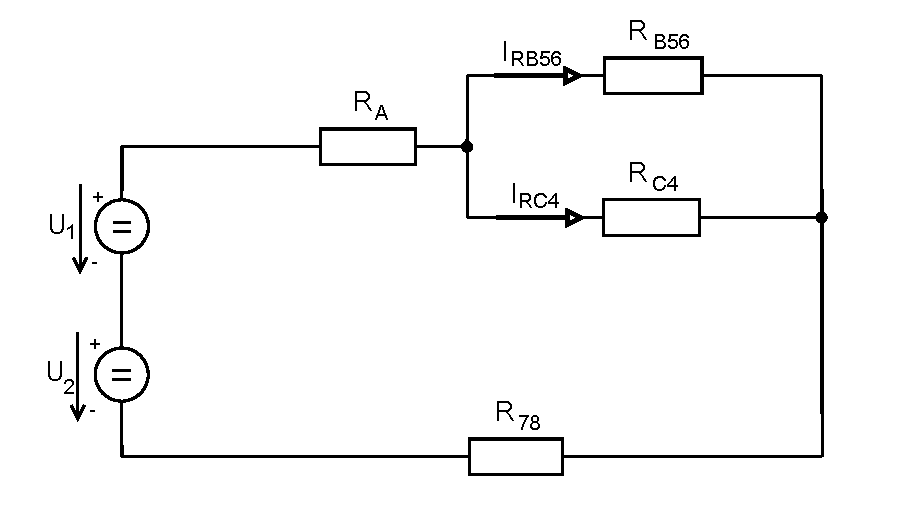
\includegraphics[scale=0.75,keepaspectratio]{xbednar00/zdroje/pr1/pr1_krok7.pdf}
\end{center}
$$U_{R_{BC456}}=U_{R_{B56}=U_{R_{C4}}}$$\\
$$I_{R_{B56}}=\frac{U_{R_{BC456}}}{R_{B56}}\doteq0,1354A$$\\
$$I_{R_{C4}}=\frac{U_{R_{BC456}}}{R_{C4}}\doteq0,0858A$$

\newpage
\subsection*{8. krok}
Kedže teraz už poznáme prúd $I_{R_{C4}}$, tak môžeme dopočítať napätie na rezistore $R_C$.
\begin{center}
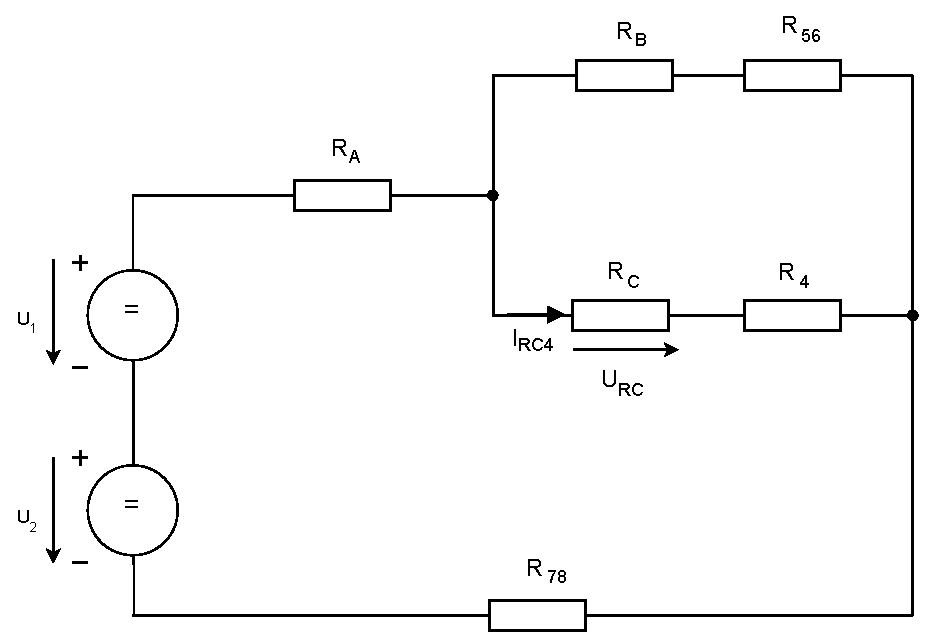
\includegraphics[scale=0.7,keepaspectratio]{xbednar00/zdroje/pr1/pr1_krok8.pdf}
\end{center}
$$U_{R_C}=I_{R_{C4}}*R_C\doteq16,0379V$$\\

\subsection*{9. krok}
Na záver vypočítame napätie $\pmb{U_{R_2}}$ a prúd $\pmb{I_{R_2}}$.
\begin{center}
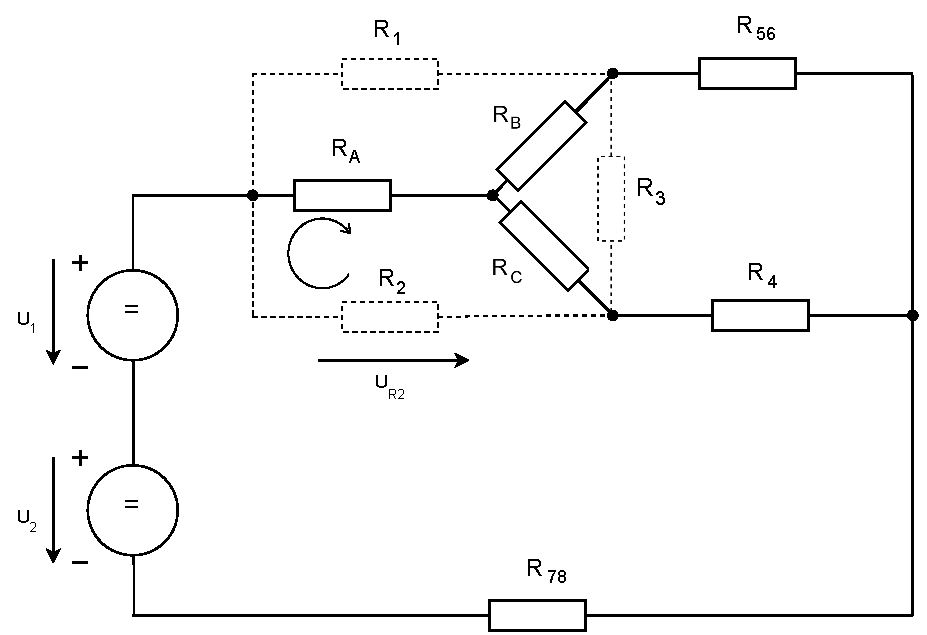
\includegraphics[scale=0.7,keepaspectratio]{xbednar00/zdroje/pr1/pr1_krok9.pdf}
\end{center}
$$U_{R_A}+U_{R_C}-U_{R_2}=0$$
$$\pmb{U_{R_2}}=U_{R_A}+U_{R_C}\doteq\pmb{68,6601V}$$
$$\pmb{I_{R_2}}=\frac{U_{R_2}}{R_2}\doteq\pmb{0,0701A}$$